% Ce fichier est inclus dans main.tex
% Ne pas compiler directement - utiliser main.tex

\chapter{Implémentation et Résultats}

\section{Introduction}

Ce chapitre décrit l'implémentation concrète du système : infrastructure Docker Compose, backend FastAPI, frontend Streamlit, intégration Groq, vector store ChromaDB, et workflows RAG avec LangChain/LangGraph. L'approche privilégie l'utilisation de LLMs hébergés via API plutôt qu'un fine-tuning local, permettant une mise en production rapide et une scalabilité accrue.

\section{Infrastructure et Déploiement}

\subsection{Docker Compose}
Quatre services principaux :
\begin{itemize}
    \item \textbf{postgres} : base de données relationnelle (utilisateurs, chats, documents).
    \item \textbf{chromadb} : vector store persistant pour les embeddings.
    \item \textbf{backend} : FastAPI (dossier \texttt{backend\_2}) exposant les endpoints.
    \item \textbf{frontend} : Streamlit (port 8502) consommant l'API backend.
\end{itemize}
Variables clés : \texttt{GROQ\_API\_KEY*}, \texttt{DATABASE\_URL}, \texttt{BACKEND\_URL}, clés optionnelles (OpenAI, Google, Tavily).

\subsection{Volumes et persistance}
\begin{itemize}
    \item \texttt{postgres\_data} pour PostgreSQL.
    \item \texttt{./data/chroma\_db} pour ChromaDB.
    \item Montages des répertoires \texttt{backend\_2} et \texttt{frontend\_streamlit} pour faciliter le développement.
\end{itemize}

\subsection{Pourquoi Docker est essentiel pour ce projet}

Docker est un choix stratégique dans notre architecture parce qu'il :
\begin{itemize}
    \item assure la portabilité entre les machines des développeurs, l'intégration continue et l'infrastructure de production,
    \item évite les conflits de dépendances (versions de Python, paquets, services système),
    \item permet d'isoler chaque service (backend, frontend, PostgreSQL, ChromaDB) pour limiter les effets de bord,
    \item facilite la montée en charge et le déploiement sur des plateformes cloud (Kubernetes, Docker Swarm, Heroku). 
\end{itemize}

Ce projet utilise un seul fichier `docker-compose.yml` pour orchestrer tous les services, ce qui rend le lancement, l'arrêt et la surveillance des logs simple et reproductible.

\section{Structure du projet}

\subsection{Backend (\texttt{backend\_2/})}
\begin{itemize}
    \item \textbf{\texttt{main.py}} : point d'entrée FastAPI.
    \item \textbf{\texttt{routes/}} : \texttt{auth.py}, \texttt{users.py}, \texttt{docs.py}, \texttt{chat.py}, \texttt{rag\_graph.py}, \texttt{rag\_langgraph.py}, \texttt{llm.py}, \texttt{llm\_graph.py}.
    \item \textbf{\texttt{models/}} : \texttt{models.py} (Pydantic \& init DB), \texttt{database.py}, \texttt{config.py}, \texttt{groq\_manager.py}, embeddings.
    \item \textbf{\texttt{auth/}} : JWT, oauth2, hachage (PBKDF2-SHA512, 25k itérations).
    \item \textbf{\texttt{data/}} : stockage fichiers/embeddings (volume).
\end{itemize}

\subsection{Frontend (\texttt{frontend\_streamlit/})}
\begin{itemize}
    \item \textbf{\texttt{app.py}} : point d'entrée Streamlit.
    \item \textbf{\texttt{components/}} : sidebar, llm\_chat, uploader, document\_list, main\_app, etc.
    \item \textbf{\texttt{pages/}} : login, signup, exam\_generation, exam\_taking, models\_info, groq\_models\_info, diagrams.
    \item \textbf{\texttt{data/}} : curriculum marocain, traductions, données pédagogiques.
    \item \textbf{\texttt{utils/}} : traductions et helpers.
\end{itemize}

\section{Backend FastAPI (backend\_2)}

\subsection{Principales dépendances}
FastAPI, SQLAlchemy/psycopg2 pour PostgreSQL, passlib (PBKDF2-SHA512, 25k itérations), LangChain/LangGraph, Chroma client, intégration Groq.

\subsection{Modèles et persistance}
Tables : \texttt{users}, \texttt{chats}, \texttt{messages}, \texttt{documents}. Les messages stockent le texte et les métadonnées; les documents stockent nom, type, chemin et état d'indexation.

\subsection{Routes et endpoints}
\begin{itemize}
    \item \textbf{Auth} : \texttt{/auth/login}, \texttt{/auth/register}, \texttt{/users/me}. JWT, mots de passe hashés PBKDF2-SHA512 (25k itérations).
    \item \textbf{Documents} : \texttt{/docs/upload}, \texttt{/docs/upload\_for\_chat} (asynchrone non bloquant), \texttt{/docs/list}, \texttt{/docs/delete/\{id\}}, \texttt{/docs/status/\{id\}}, \texttt{/docs/files/\{id\}}.
    \item \textbf{Chats} : \texttt{/chats/list}, \texttt{/chats/create}, \texttt{/chats/\{id\}/messages}, \texttt{/chats/\{id\}/add\_message}.
    \item \textbf{LLM/RAG} : \texttt{/rag\_langgraph2} (RAG avec LangGraph), \texttt{/llm\_groq\_graph} (chat simple Groq).
\end{itemize}

\subsection{Synthèse (usage applicatif)}
\begin{itemize}
    \item \textbf{Auth} : inscription / login via JWT, récupération du profil courant.
    \item \textbf{Documents} : upload + indexation asynchrone, liste/suppression, suivi d'état, téléchargement.
    \item \textbf{Chats} : création, ajout et lecture des messages d'un chat.
    \item \textbf{IA} : \texttt{/rag\_langgraph2} (RAG filtré par documents sélectionnés), \texttt{/llm\_groq\_graph} (chat général Groq).
\end{itemize}

\subsection{Gestion des documents et RAG}
\begin{itemize}
    \item Upload : enregistrement DB immédiat, traitement asynchrone (extraction texte, chunking).
    \item Indexation : stockage des embeddings dans ChromaDB avec \texttt{document\_id}; filtrage par document sélectionné.
    \item Fallback : si la recherche sémantique est vide, récupération complète des chunks du document sélectionné.
\end{itemize}

\subsection{Intégration Groq}
Sélection de modèles côté frontend, transmis au backend :
\begin{itemize}
    \item \texttt{llama-3.1-8b-instant} (rapide/économique)
    \item \texttt{llama-3.3-70b-versatile} (généraliste)
    \item \texttt{qwen/qwen3-32b} (multilingue, 128k contexte)
    \item \texttt{openai/gpt-oss-20b} (très haut débit)
    \item \texttt{openai/gpt-oss-120b} (grande capacité)
    \item \texttt{deepseek-r1-distill-llama-70b} (déprécié sur Groq)
\end{itemize}

\section{Frontend Streamlit}

\subsection{Navigation et pages}
\begin{itemize}
    \item \textbf{Home} : présentation PFE, actions rapides.
    \item \textbf{Chat} : tuteur IA (RAG ou simple), sélection modèle Groq, sujet/niveau/cours, instructions personnalisées, langue (FR/EN/AR).
    \item \textbf{Upload / Documents} : upload multi-fichiers, liste, suppression.
    \item \textbf{Generate Exam} : génération d'examens (JSON/PDF/DOCX), distribution par cours, multilingue, boutons d'export.
    \item \textbf{Take Exam} : chargement d'examen (JSON/PDF/DOCX), réponses, feedback détaillé, export résultats.
    \item \textbf{Models Info / Groq Pricing} : fiches modèles, benchmarks et tarifs Groq.
    \item \textbf{Diagrams} : schémas de base de données et workflow pour documentation.
\end{itemize}

\subsection{Multilingue et prompts}
La langue choisie dans la sidebar (FR, EN, AR) est propagée aux prompts (chat, génération d'examens, feedback). Les prompts de génération d'examens imposent la langue pour titres, questions, réponses et noms de cours.

\subsection{Composants clés}
Sidebar (langue, modèle, sujet/niveau/cours, instructions), chat RAG (sélection de documents, boutons rapides exercice/cours), uploader, liste de documents, pages d'examens.

\section{Schémas (base de données et workflow)}

\subsection{Schéma conceptuel de base de données}
Le système utilise une base de données relationnelle PostgreSQL avec les tables suivantes :
\begin{itemize}
    \item \texttt{users} : authentification et profils utilisateurs (id, login, password, team\_id, role, is\_active, created\_at, updated\_at)
    \item \texttt{chats} : conversations utilisateurs (chat\_id, user\_id, chat\_title, chat\_type, created\_at)
    \item \texttt{chat\_messages} : messages dans les conversations (message\_id, chat\_id, role, content, timestamp)
    \item \texttt{documents} : métadonnées des documents uploadés (doc\_id, user\_id, team\_id, doc\_title, file\_type, visibility, upload\_date, file\_path)
    \item \texttt{prompt\_templates} : modèles de prompts réutilisables (id, title, content, type, tags[], visibility, team\_id, created\_by, created\_at)
\end{itemize}

Relations principales : \texttt{users} $\rightarrow$ \texttt{chats} (1..n), \texttt{users} $\rightarrow$ \texttt{documents} (1..n), \texttt{users} $\rightarrow$ \texttt{prompt\_templates} (1..n), \texttt{chats} $\rightarrow$ \texttt{chat\_messages} (1..n).

Pour illustrer ce schéma conceptuel dans le rapport, nous réservons l'emplacement suivant où sera insérée la capture d'écran du diagramme Streamlit :

\begin{figure}[h]
    \centering
    % Remplacer le nom de fichier ci-dessous par l'image exportée depuis la page "Diagrams"
    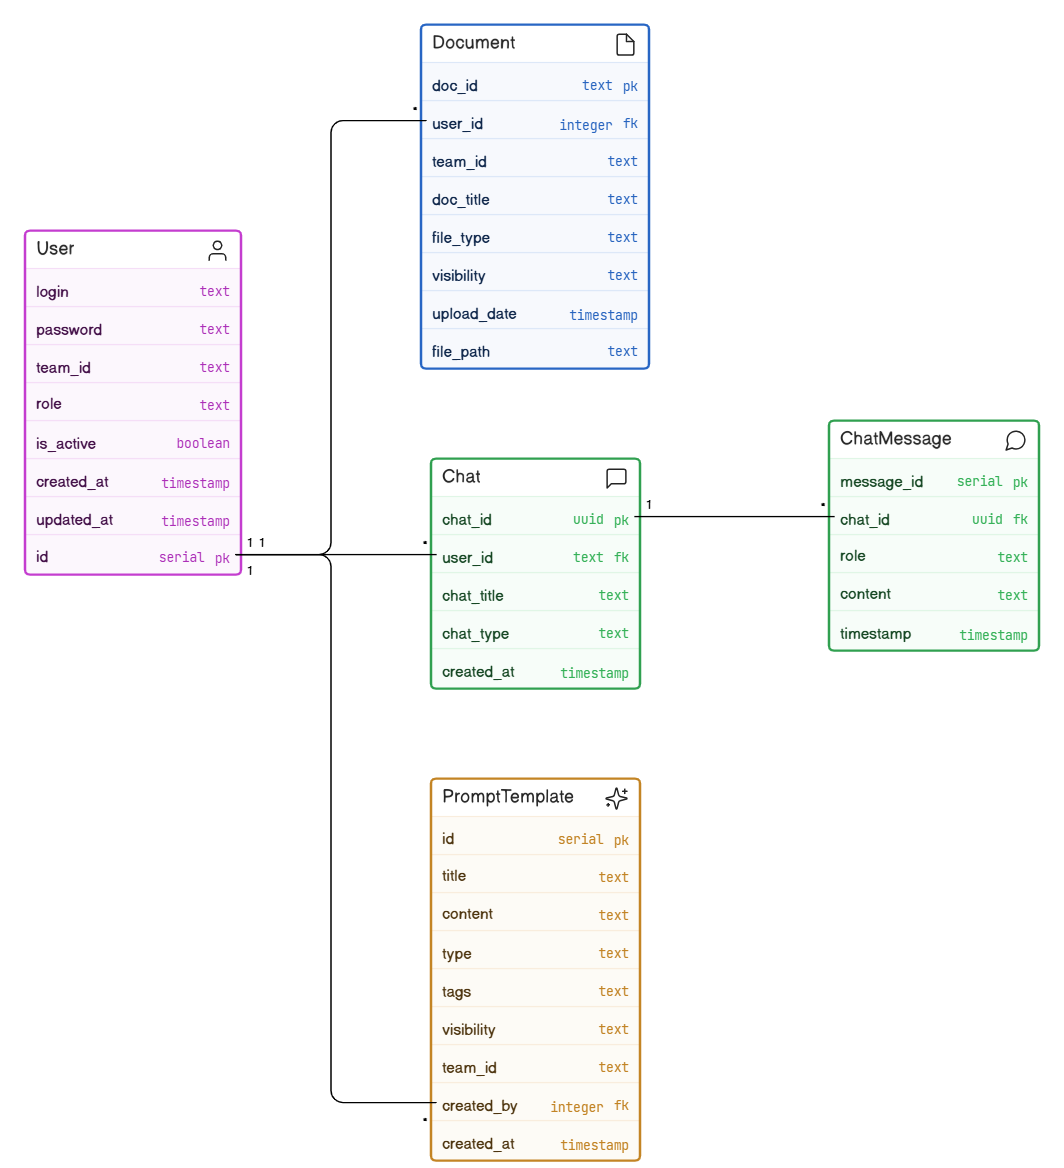
\includegraphics[width=0.95\textwidth]{images/class diagram2.png}
    \caption{Schéma conceptuel de la base de données du système.}
    \label{fig:schema-bd-conceptuel}
\end{figure}

\subsection{Workflow global (simplifié)}
Le flux principal suit ces étapes :
\begin{enumerate}
    \item \textbf{Authentification} : l'utilisateur se connecte via \texttt{/auth/login} et reçoit un token JWT.
    \item \textbf{Upload de documents} : l'utilisateur upload des fichiers via \texttt{/docs/upload\_for\_chat}; le backend enregistre les métadonnées en DB et lance un traitement asynchrone (extraction, chunking, indexation ChromaDB).
    \item \textbf{Recherche contextuelle} : lors d'un chat RAG (\texttt{/rag\_langgraph2}), le système recherche dans ChromaDB les chunks pertinents filtrés par \texttt{document\_id} sélectionné.
    \item \textbf{Génération IA} : le contexte récupéré est injecté dans un prompt système; le modèle Groq sélectionné génère la réponse.
    \item \textbf{Génération d'examens} : le frontend construit un prompt détaillé avec distribution par cours; le backend appelle Groq pour générer l'examen en JSON; export PDF/DOCX optionnel.
    \item \textbf{Correction automatique} : lors du passage d'examen, chaque réponse est évaluée par le LLM; feedback par question et global générés; export des résultats.
\end{enumerate}

Le workflow global affiché dans l'application (page ``Diagrams'') est également intégré au rapport sous forme d'image. L'emplacement ci-dessous sert de placeholder pour la capture d'écran correspondante :

\begin{figure}[h]
    \centering
    % Remplacer le nom de fichier ci-dessous par l'image exportée depuis la page "Diagrams"
    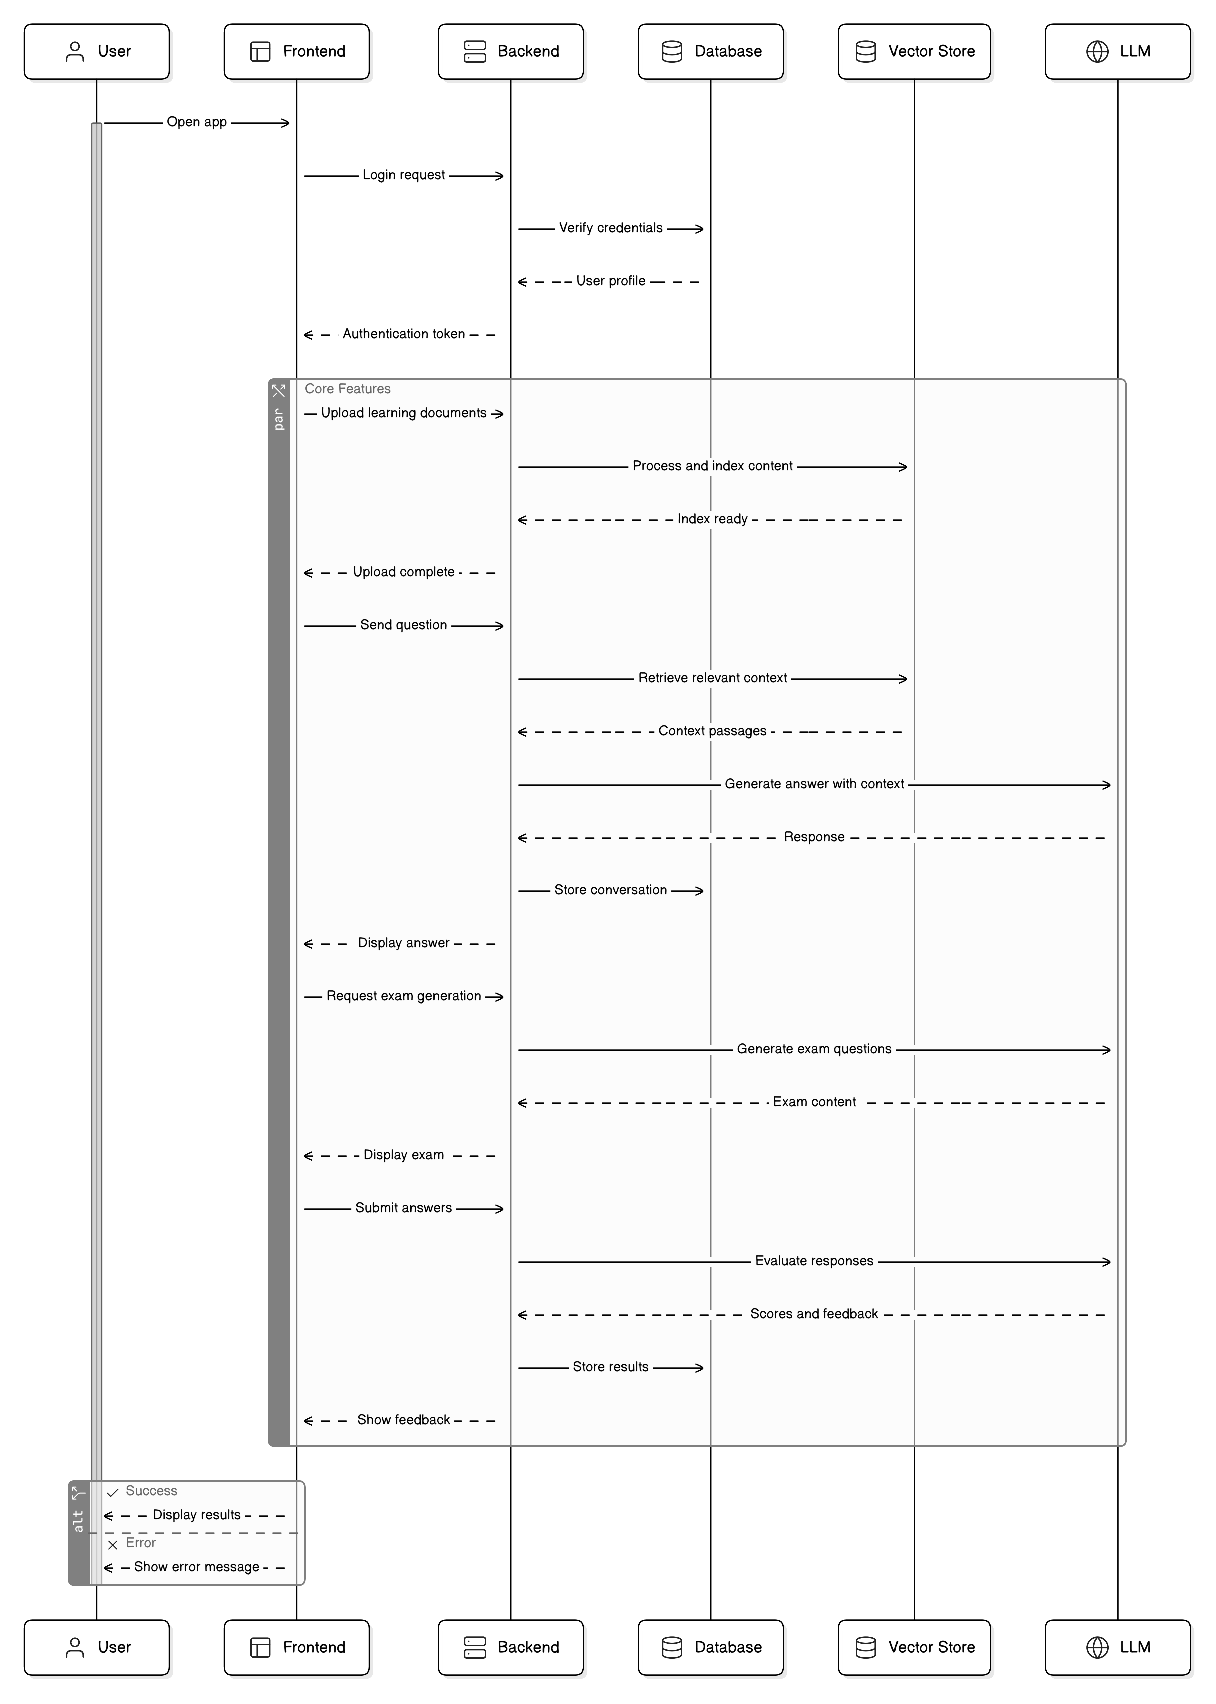
\includegraphics[width=0.95\textwidth]{images/diagram-export.png}
    \caption{Workflow global simplifié du système (du point de vue utilisateur $\rightarrow$ backend $\rightarrow$ Groq/ChromaDB).}
    \label{fig:workflow-global}
\end{figure}

\section{Workflows RAG (LangChain / LangGraph)}
\begin{itemize}
    \item Conversion de l'historique en messages LangChain.
    \item Recherche ChromaDB filtrée par \texttt{document\_id}; fallback complet du document si nécessaire.
    \item Prompt système flexible : accepte tout type de document (pas seulement maths).
    \item Génération via modèle Groq sélectionné; fallback RAG simple en cas d'échec LangGraph.
\end{itemize}

\section{Fonctionnalités Pédagogiques}

Cette section détaille le processus complet de génération, upload, extraction, validation et feedback des examens, qui constitue le cœur pédagogique du système.

\subsection{Génération d'examens}
% capture d'écran de la page de génération d'examen — étape 1
\begin{figure}[H]
    \centering
    \includegraphics[width=0.8\textwidth]{images/CreationExamen1.png}
    \caption{Page de création d'examen — étape 1.}
    \label{fig:creation-examen-1}
\end{figure}

% capture d'écran de la page de génération d'examen — étape 2
\begin{figure}[H]
    \centering
    \includegraphics[width=0.8\textwidth]{images/CreationExamen2.png}
    \caption{Page de création d'examen — étape 2.}
    \label{fig:creation-examen-2}
\end{figure}
Le système permet de générer automatiquement des examens personnalisés via des LLMs Groq. Le processus suit les étapes suivantes :

\textbf{Configuration de l'examen :}
\begin{enumerate}
    \item L'enseignant sélectionne le \textbf{niveau} (collège/lycée), la \textbf{matière} (mathématiques, physique, etc.), et la \textbf{difficulté} (Facile, Intermédiaire, Difficile).
    \item Il choisit les \textbf{cours/thèmes} à couvrir et définit une \textbf{distribution par pourcentage} (ex: 30\% Algèbre, 40\% Géométrie, 30\% Calcul).
    \item Il spécifie le \textbf{nombre total de questions} et la \textbf{langue} de génération (FR/EN/AR).
    \item Optionnellement, il peut demander l'inclusion des \textbf{réponses modèles} pour chaque question.
\end{enumerate}



\textbf{Génération via LLM :}
Le frontend construit un prompt structuré contenant toutes les spécifications et l'envoie au backend, qui appelle l'API Groq avec le modèle sélectionné. Le prompt inclut :
\begin{itemize}
    \item Les métadonnées (niveau, matière, difficulté, langue)
    \item La distribution exacte par cours (nombre de questions par cours)
    \item Des instructions strictes pour garantir l'unicité des questions (éviter les répétitions)
    \item Le format de sortie JSON attendu avec structure : \texttt{title}, \texttt{subject}, \texttt{grade}, \texttt{questions[]} (chacune avec \texttt{course}, \texttt{question}, \texttt{answer} optionnel, \texttt{difficulty})
\end{itemize}

Le LLM génère l'examen complet en respectant la distribution et la langue imposées. Le système vérifie l'unicité des questions générées (détection de similarité) et peut régénérer si nécessaire.

\textbf{Export multi-format :}
L'examen généré peut être exporté en :
\begin{itemize}
    \item \textbf{JSON} : format natif pour réutilisation dans le système
    \item \textbf{PDF} : document formaté avec ReportLab, prêt pour impression
    \item \textbf{DOCX} : document Word éditable avec python-docx
\end{itemize}

\subsection{Upload et extraction d'examens}

Les enseignants peuvent également uploader des examens existants (JSON, PDF, ou DOCX) plutôt que de les générer.

\textbf{Upload de fichiers :}
\begin{itemize}
    \item \textbf{JSON} : format natif, chargement direct sans traitement
    \item \textbf{PDF} : extraction de texte via PyPDF2, parsing des questions
    \item \textbf{DOCX} : extraction de texte via python-docx, parsing des questions
\end{itemize}

\textbf{Extraction des questions :}
Le système utilise deux méthodes d'extraction selon le format :

\textit{Méthode 1 - Pattern Matching (pour PDF/DOCX) :}
\begin{itemize}
    \item Détection de patterns comme ``Question N'', ``Cours: X | Difficulté: Y'', numérotation (1., 2., etc.)
    \item Nettoyage automatique : suppression des lignes avec underscores (\_\_\_\_), lignes ``Réponse:'', lignes vides
    \item Extraction des métadonnées (cours, difficulté) si présentes dans le document
    \item Regroupement du texte de chaque question en objets structurés
\end{itemize}

\textit{Méthode 2 - Extraction par LLM (optionnelle, pour documents complexes) :}
\begin{itemize}
    \item Le contenu textuel est envoyé à un LLM Groq avec un prompt spécialisé d'extraction
    \item Le prompt demande d'identifier \textbf{toutes} les questions, de les séparer individuellement, de déterminer le cours/thème et la difficulté pour chacune
    \item Le LLM retourne un JSON structuré avec la liste complète des questions extraites
    \item Cette méthode est plus robuste pour les documents avec formatage complexe ou structures non standard
\end{itemize}

Le résultat de l'extraction est normalisé au même format JSON que les examens générés, permettant un traitement uniforme par la suite.
% capture d'écran de la page
\begin{figure}[H]
    \centering
    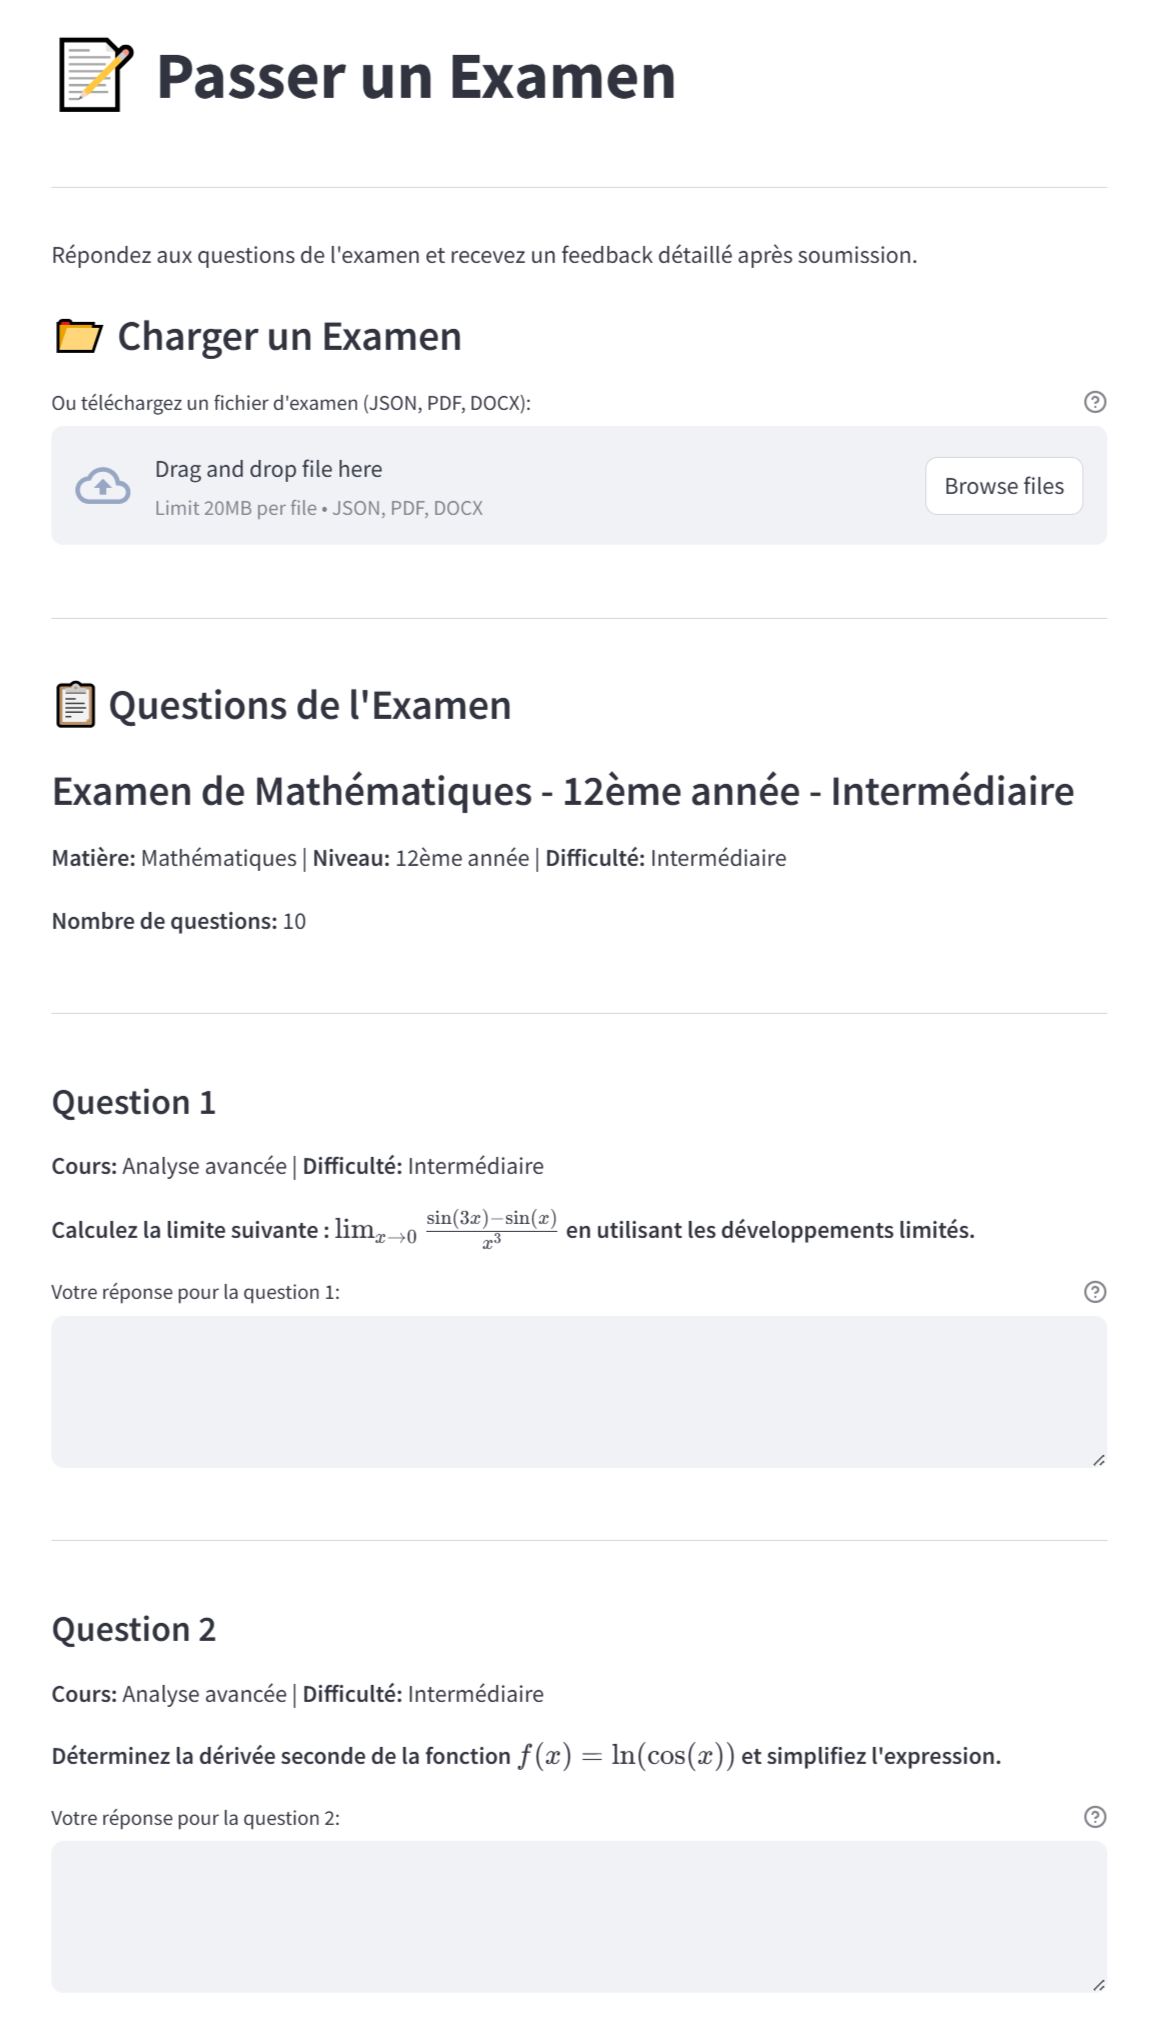
\includegraphics[width=0.7\textwidth]{images/PasserunExamen.png}
    \caption{Page de  Passer un Examen.}
    \label{fig:creation-examen-2}
\end{figure}
\subsection{Validation et notation par IA}

Une fois l'examen chargé (généré ou uploadé) et les réponses de l'élève saisies, le système procède à la validation automatique via LLM.

\textbf{Classification par question :}
Pour chaque question, le système :
\begin{enumerate}
    \item Construit un prompt de classification contenant :
    \begin{itemize}
        \item L'énoncé de la question
        \item La réponse de l'élève
        \item Le contexte (matière, niveau, cours)
        \item Des instructions pour classifier en : \textbf{correcte}, \textbf{partiellement correcte}, ou \textbf{incorrecte}
    \end{itemize}
    \item Appelle le backend qui invoque le LLM Groq sélectionné (via endpoint \texttt{/rag\_langgraph2} ou \texttt{/llm\_groq\_graph})
    \item Le LLM analyse la réponse et retourne un JSON avec :
    \begin{itemize}
        \item \texttt{classification} : ``correcte'', ``partiellement correcte'', ou ``incorrecte''
        \item \texttt{feedback} : explication détaillée et pédagogique (pourquoi correcte/partielle/incorrecte, suggestions d'amélioration)
    \end{itemize}
    \item Le prompt de classification est multilingue (FR/EN/AR) selon la langue sélectionnée par l'utilisateur
\end{enumerate}

\textbf{Calcul de la note :}
Le système calcule automatiquement le score final selon la formule :
\begin{equation}
\text{Score} = \frac{\text{Nombre de réponses correctes} + 0.5 \times \text{Nombre de réponses partielles}}{\text{Nombre total de questions}} \times 100\%
\end{equation}

Les réponses incorrectes ou absentes comptent pour 0 point. Le score est affiché avec un code couleur (vert $\geq$ 70\%, orange $\geq$ 50\%, rouge $<$ 50\%).

\subsection{Génération de feedback}

Le système génère deux niveaux de feedback pour guider l'élève :

\textbf{Feedback par question :}
Chaque question reçoit un feedback personnalisé généré par le LLM lors de la classification. Ce feedback :
\begin{itemize}
    \item Explique pourquoi la réponse est correcte, partiellement correcte, ou incorrecte
    \item Identifie les erreurs spécifiques commises (calculs incorrects, concepts mal compris, etc.)
    \item Propose des suggestions d'amélioration et des pistes de remédiation
    \item S'adapte au niveau et à la matière (langage pédagogique approprié)
\end{itemize}

\textbf{Feedback global :}
Après le calcul du score, le système génère un feedback global synthétique via LLM. Le prompt inclut :
\begin{itemize}
    \item Le score final obtenu
    \item Le nombre de questions correctes, partielles, et incorrectes
    \item La matière et le niveau
    \item Des instructions pour générer un feedback encourageant et constructif
\end{itemize}

Le feedback global :
\begin{itemize}
    \item Synthétise les points forts de l'élève
    \item Identifie les difficultés récurrentes (par cours/thème si possible)
    \item Propose un plan d'amélioration ciblé
    \item Encourage la progression (ton adapté au score)
\end{itemize}

\textbf{Export des résultats :}
Les résultats complets (questions, réponses, classifications, feedbacks individuels, score, feedback global) peuvent être exportés en PDF ou DOCX pour archivage ou partage avec l'enseignant.

\subsection{Tuteur IA interactif}

En complément des examens, le système offre un mode tuteur IA interactif :
\begin{itemize}
    \item \textbf{Mode RAG} : l'élève peut poser des questions sur des documents uploadés; le système récupère le contexte pertinent via ChromaDB et génère des réponses contextualisées
    \item \textbf{Mode chat simple} : conversation libre avec le LLM Groq sans documents (pour questions générales, explications de concepts)
    \item \textbf{Historique persistant} : toutes les conversations sont sauvegardées en base (table \texttt{chats} et \texttt{chat\_messages}) pour continuité pédagogique
    \item \textbf{Boutons rapides} : depuis le chat, l'élève peut demander la génération d'un exercice ou d'un cours sur un thème spécifique
\end{itemize}

\section{Tests et Résultats}

\subsection{Protocole d'évaluation}

Les tests fonctionnels ont été réalisés selon un protocole structuré :

\textbf{Environnement de test :}
\begin{itemize}
    \item Infrastructure : Docker Compose local (backend, frontend, PostgreSQL, ChromaDB)
    \item Modèles testés : llama-3.1-8b-instant, llama-3.3-70b-versatile, qwen/qwen3-32b
    \item Documents d'essai : PDFs pédagogiques (mathématiques, physique), DOCX de cours, fichiers texte
    \item Langues testées : Français, English, العربية
\end{itemize}

\textbf{Scénarios de test :}
\begin{enumerate}
    \item \textbf{Upload \& indexation} : upload de fichiers PDF/DOCX/TXT, vérification du statut d'indexation via \texttt{/docs/status/\{id\}}, listing via \texttt{/docs/list}, suppression.
    \item \textbf{RAG contextualisé} : sélection d'un document, envoi de questions, vérification que les réponses utilisent le contexte du document (test avec documents non mathématiques pour valider la flexibilité des prompts).
    \item \textbf{Génération d'examens} : création d'examens avec distribution par cours (ex: 1 question "Nombres entiers", 2 questions "Opérations de base", 2 questions "Géométrie"), vérification du respect de la distribution, export JSON/PDF/DOCX, validation de la langue (FR/EN/AR).
    \item \textbf{Passage d'examens} : chargement d'examen (JSON/PDF/DOCX), saisie de réponses, génération de feedback par question et global, export des résultats.
    \item \textbf{Chat multilingue} : changement de langue dans la sidebar, vérification que les réponses et les prompts d'examen respectent la langue sélectionnée.
\end{enumerate}

\subsection{Résultats fonctionnels}

\textbf{Upload \& indexation :}
\begin{itemize}
    \item Tous les formats testés (PDF, DOCX, TXT) sont correctement traités.
    \item L'indexation asynchrone fonctionne sans bloquer l'interface utilisateur.
    \item Le statut d'indexation est correctement suivi et affiché.
    \item Temps moyen d'indexation : 2-5 secondes pour un document de 10 pages.
\end{itemize}

\textbf{RAG :}
\begin{itemize}
    \item Les réponses sont contextualisées sur les documents sélectionnés.
    \item Le système fonctionne avec des documents non mathématiques (test avec CV, lettres) grâce aux prompts flexibles.
    \item Le fallback (récupération complète des chunks si recherche vide) fonctionne correctement.
    \item Latence moyenne : 3-8 secondes selon le modèle (8b-instant plus rapide que 70b-versatile).
\end{itemize}

\textbf{Génération d'examens :}
\begin{itemize}
    \item La distribution par cours est respectée (ex: 1+2+2 = 5 questions totales).
    \item Les examens générés sont cohérents avec le niveau et la matière sélectionnés.
    \item L'export multi-format (JSON/PDF/DOCX) fonctionne correctement.
    \item La langue est correctement appliquée (titres, questions, réponses en FR/EN/AR selon sélection).
\end{itemize}

\textbf{Passage d'examens et feedback :}
\begin{itemize}
    \item Le chargement d'examens depuis JSON/PDF/DOCX fonctionne.
    \item Le feedback par question identifie correctement les réponses correctes, partielles et incorrectes.
    \item Le feedback global synthétise les points forts et les difficultés.
    \item L'export des résultats (JSON/PDF/DOCX) est opérationnel.
\end{itemize}

\textbf{Multilingue :}
\begin{itemize}
    \item Le changement de langue dans la sidebar est immédiatement reflété dans l'interface.
    \item Les réponses du chat respectent la langue sélectionnée.
    \item Les examens générés sont dans la langue choisie (titres, questions, réponses).
    \item Les trois langues (FR/EN/AR) sont correctement supportées.
\end{itemize}

\subsection{Limitations identifiées}

\begin{enumerate}
    \item \textbf{Robustesse RAG} : dépend de la qualité des documents uploadés et de l'indexation; améliorable par reranking pour améliorer la pertinence des contextes récupérés.
    \item \textbf{Coût LLM} : le choix du modèle (8B vs 70B vs 120B) impacte vitesse, coût et qualité; sélection automatique selon la tâche serait bénéfique.
    \item \textbf{Détection fine des compétences} : la classification des erreurs (correct/partiel/incorrect) pourrait être affinée avec des jeux de réponses plus variés pour mieux identifier les difficultés récurrentes.
    \item \textbf{Latence} : les modèles plus grands (70B, 120B) sont plus lents; acceptable pour la génération d'examens mais peut impacter l'expérience chat en temps réel.
\end{enumerate}

\section{Conclusion du Chapitre}

Ce chapitre a présenté l'implémentation complète du système basé sur des LLMs hébergés via API Groq, une architecture microservices containerisée, et des workflows RAG avec LangChain/LangGraph. Les tests fonctionnels confirment que :

\begin{enumerate}
    \item L'architecture FastAPI/Streamlit/PostgreSQL/ChromaDB est opérationnelle et scalable.
    \item Le RAG fonctionne correctement avec filtrage par document et fallback robuste.
    \item La génération et le passage d'examens sont fonctionnels avec support multilingue.
    \item Les limitations identifiées (reranking, sélection automatique de modèle, affinement de la détection d'erreurs) constituent des pistes d'amélioration futures.
\end{enumerate}

L'approche privilégiant des LLMs hébergés plutôt qu'un fine-tuning local permet une mise en production rapide, une maintenance simplifiée, et une scalabilité accrue. Le chapitre suivant présentera la conclusion générale du projet et les perspectives futures.
